\documentclass{article}

\usepackage[utf8]{inputenc}
\usepackage[T1]{fontenc}
\usepackage[frenchb]{babel}
\usepackage[top=2cm, bottom=2cm, left=3cm, right=3cm]{geometry}
\usepackage{hyperref}
\usepackage{graphicx}
\usepackage{fancyhdr}
\usepackage{fancybox}

\hypersetup{colorlinks=true}

\title{Snakekans\\-- Projet ISN --}
\author{Luc Chabassier <\href{mailto:luc.linux@mailoo.org}{\nolinkurl{luc.linux@mailoo.org}}> \and Pablo Donato <\href{mailto:pablo.donato@mailoo.org}{\nolinkurl{pablo.donato@mailoo.org}}>}

\begin{document}
\maketitle

\tableofcontents

\section{Introduction.}
Ce programme doit être créé dans le cadre d'un projet d'ISN en 2013. L'idée initiale est de faire un snake en réseau (deux joueurs).

\section{Fonctionnalités.}
Contrairement à l'idée initiale, le jeu est finalement capable de gérer jusqu'à quatre joueurs en local, en connectant des joysticks. L'idée du réseau est conservée : un des joueurs sera le serveurs, et donc effectuera la majorité des calculs, et des joueurs devront pouvoir se connecter à lui.

Le jeu s'organise sur une grille virtuelle composée de case de 20 pixels sur 20 pixels.

\subsection{Règles du jeu.}
Le programme est un snake classique, c'est à dire que le terrain ne contient que les serpents et les bonus. Quand un serpent sort d'un côté, il entre de l'autre. Les bonus apportent un certain nombre de points chacun. Le jeu se termine quand un des serpents meurt, c'est à dire qu'il se cogne contre un autre des serpents ou contre lui-même. Le gagnant est celui qui a le plus de points. Afin de dévaloriser la mort, chaque serpent a un malus en fonction du nombre de serpents restants quand il meurt.

S'il y a plusieurs joueurs, le jeu se termine quand n'y n'en reste plus qu'un vivant. S'il n'y a qu'un seul joueur, le jeu se termine à sa mort.

\subsection{TODO liste.}
\begin{description}
	\item[Terminé :] \begin{itemize}
			\item Chargement et affichage du serpent.
			\item Chargement des bonus.
			\item Collisions.
			\item Écran de game over.
			\item Menu principal.
			\item Gestion des joysticks.
			\item Écran de sélection des joueurs.
			\item Musique et sons.
		\end{itemize}
	\item[À faire :] \begin{itemize}
			\item Le réseau.
			\item Écran de connexion.
		\end{itemize}
\end{description}

\subsection{Les bonus.}
Un bonus possède plusieurs attributs. Tout d'abord, le nombre de points qu'il rapporte et l'influence sur la taille : un bonus peut donc faire perdre des points et/ou raccourcir le serpent. Un bonus possède aussi une durée durant laquelle il reste affiché et une probabilité d'apparition. Enfin, chaque bonus possède une image propre.

Les bonus sont stocké dans un ficher config (clé=valeur) de la forme :
\begin{verbatim}
pts = 10
length = 3 # influence for the snake length
time = 10000 # in milliseconds
picture = pictures/banana.png
fact = 20 # Higher is fact, higher is the apparition frequency
\end{verbatim}

Tous les fichiers des bonus sont dans un dossier dont le contenu est scanné au début du programme.

\subsection{Le serpent.}
Le serpent est stocké dans un structure. Il peut se déplacer dans quatre directions. Un serpent est affiché avec une succession d'images, chargée depuis un tileset. Il existe quatre image pour le serpent : la tête, un corp droit, un corp courbe et la queue. Chacune de ces images existe en deux exemplaire, qui servent à créer une animation lors du déplacement du serpent.

\subsection{Le terrain.}
Le terrain est constitué d'une image de fond, uniquement décorative. Le nombre de cases, ainsi que leur taille, est fixé dans le code. Chaque case non vide contient ou un bonus, ou une information de collision quand il y a le corp du serpent.

\section{L'interface.}
Le jeu étant encore en développement, les interfaces présentées et/ou décrites sont susceptibles d'être différentes de celles de la release du programme.

\subsection{Le menu.} \label{menu}
\begin{center}
	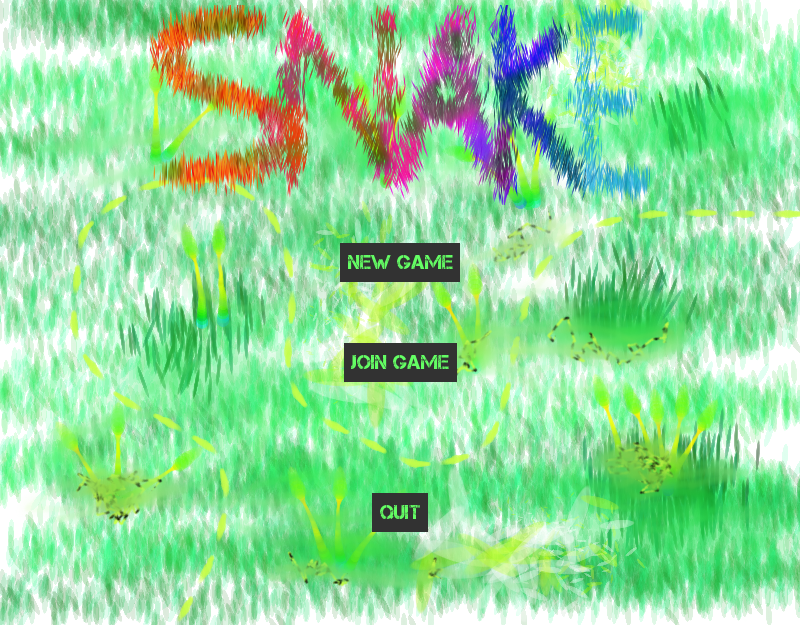
\includegraphics[scale=0.4]{img/menu.png}
\end{center}
Le menu possède trois boutons, en dessous du titre :
\begin{description}
	\item[New Game] Ce bouton permet de lancer une partie en local et/ou en serveur. Il amène à l'écran décrit en~\ref{select}.
	\item[Join Game] Ce bouton permet de rejoindre une partie créée par un New Game sur un autre ordinateur. Il lance le client réseau et amène à l'écran décrit en~\ref{connect}.
	\item[Quit] Ce bouton termine le jeu. Il a le même effet que fermer la fenêtre.
\end{description}

\subsection{La sélection des joueurs.} \label{select}
\begin{center}
	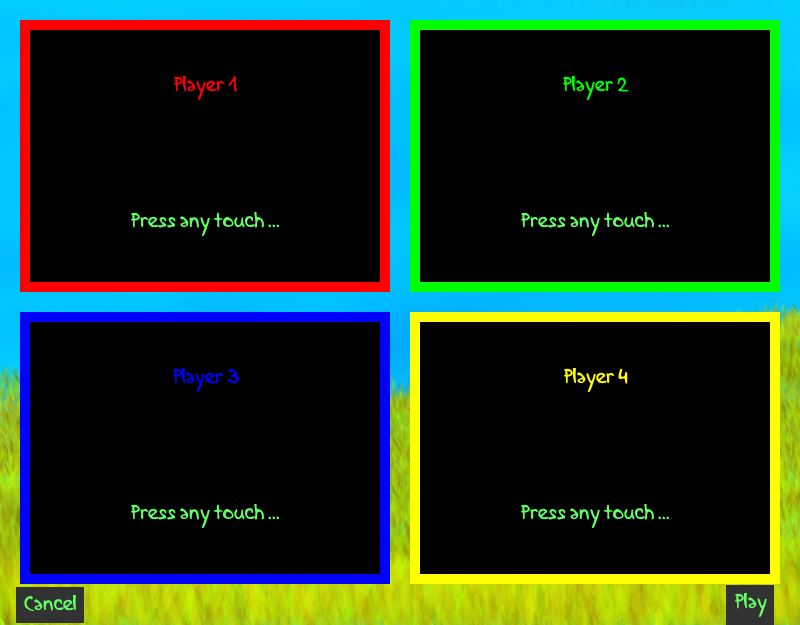
\includegraphics[scale=0.4]{img/empty.png}
\end{center}
Ce menu possède quatre case. Chaque case correspond à un joueur. Pour ajouter un joueur, il faut laisser appuyé un bouton sur le controleur (joystick ou clavier) qu'il souhaite utiliser. Les conexions de clients apparaissent aussi ici.

Ce menu avec un clavier et un joystick connecté ressemble à :
\begin{center}
	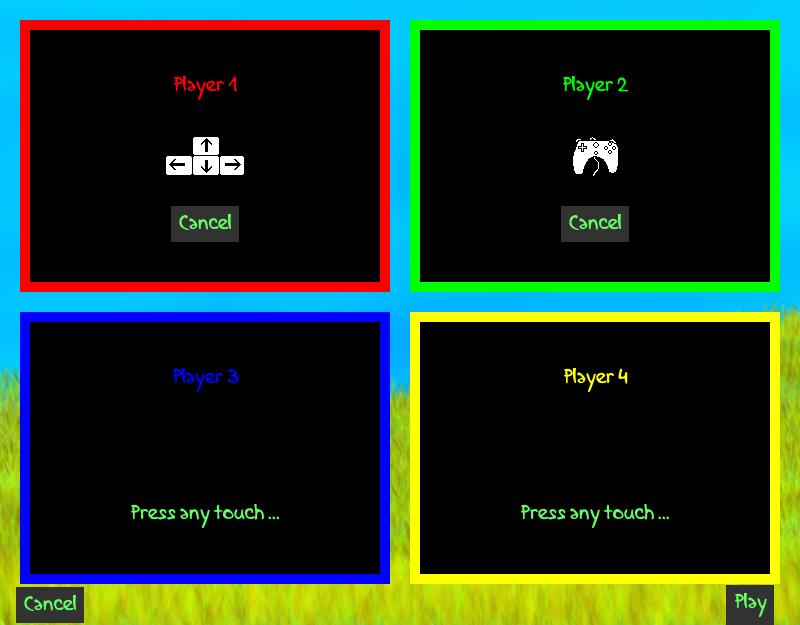
\includegraphics[scale=0.4]{img/full.png}
\end{center}

Ce menu possède deux boutons :
\begin{description}
	\item[Cancel] Ce bouton ramène au menu général, décrit en~\ref{menu}.
	\item[Play] Ce bouton lance un jeu (voir~\ref{game}) avec les joueurs connectés.
\end{description}

\subsection{La connexion.} \label{connect}
Cet écran n'a pas encore été implémenté, donc aucune image ne sera montrée.

Cet écran contient trois éléments importants : \begin{enumerate}
	\item Un champ de texte associé à un bouton \emph{Connect} qui permet d'entrer l'adresse à laquelle se connecter puis de lancer la connexion.
	\item Un cadre permettant de choisir quel contrôleur (joystick, clavier) on veut utiliser. Ce contrôleur est identique aux quatre que l'on trouve en~\ref{select}.
	\item Un bouton cancel qui permet de retourné au menu principal décrit en~\ref{menu}.
\end{enumerate}

\subsection{Le jeu.} \label{game}
\begin{center}
	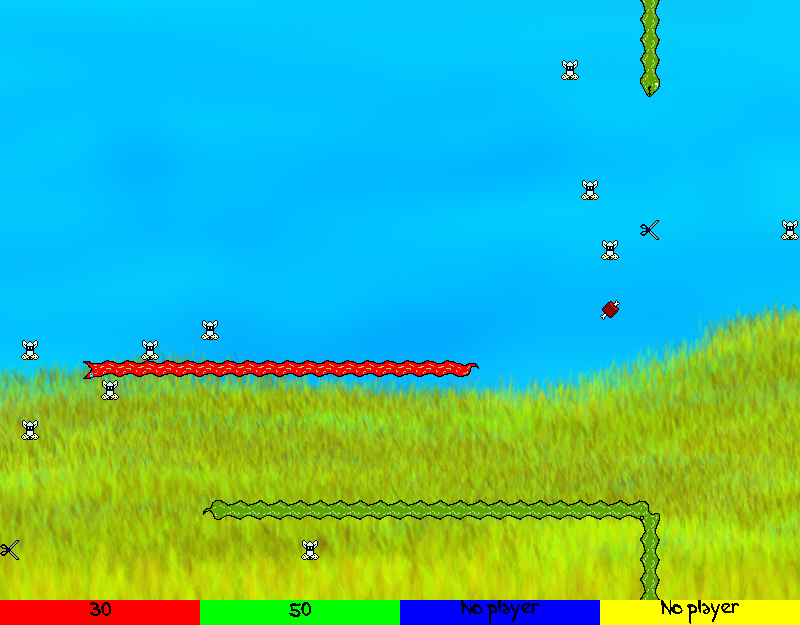
\includegraphics[scale=0.4]{img/game.png}
\end{center}
On remarque sur cette capture d'écran deux serpents, donc deux joueurs connectés, ainsi que divers bonus. En bas de l'écran se trouve la barre qui indique les score des joueurs.

Lorsque le jeu est terminé, on arrive sur cet écran :
\begin{center}
	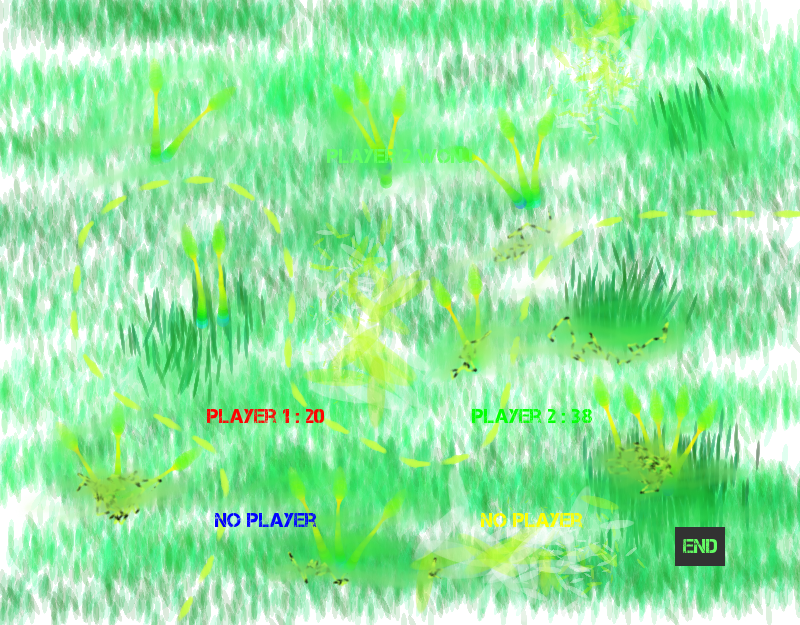
\includegraphics[scale=0.4]{img/game_over.png}
\end{center}
Cet écran affiche le score de chaque joueur ainsi que le gagnant. Le bouton \emph{End} permet de retourner à l'écran de sélection des joueurs (partie~\ref{select}) avec les joueurs connectés comme avant la partie, permettant de relancer une partie très rapidement.

\section{Développement.}
\subsection{Bibliothèques utilisées.}
Ce jeu est codé en c++, et certaines bibliothèques SDL : tout d'abord la bibliothèque \href{http://www.libsdl.org/}{SDL} de base, avec ses extensions \href{http://www.libsdl.org/projects/SDL\_image/}{SDL\_image}, \href{http://www.libsdl.org/projects/SDL\_ttf/}{SDL\_ttf} et \href{http://www.libsdl.org/projects/SDL\_mixer/}{SDL\_mixer}. Certaines bibliothèque \href{http://www.boost.org/}{boost} sont elles aussi utilisées : \href{http://www.boost.org/doc/libs/1\_39\_0/libs/filesystem/doc/index.htm}{boost.filesystem} et \href{http://www.boost.org/doc/libs/1\_53\_0/libs/regex/doc/html/index.html}{boost.regex}.

Ce cahier des charges est rédigé en \href{http://www.latex-project.org/}{\LaTeX}.

\subsection{Outils.}
L'outil utilisé pour écrire le code est \href{http://www.vim.org/}{Vim} (éditeur et colorateur). Le code est versionné avec \href{http://git-scm.com/}{git} (le code est hébergé sur \href{https://github.com/Lycee/ISN\_snake}{github}) et la chaine de compilation est générée par \href{http://www.cmake.org/}{Cmake}. Le jeu est dévellopé sous \href{https://en.wikipedia.org/wiki/Linux}{GNU/Linux} mais devra être compatible avec d'autre plateforme comme Windows ou Mac.

\section{Licence.}
Le code est sous licence \href{http://gplv3.fsf.org/}{GNU GPLv3} (voir le fichier LICENCE fournit avec le code), au copyright de Luc Chabassier et Pablo Donato.

Les ressources graphiques (images, tileset) ont été crées par Luc Chabassier à l'aide de \href{http://www.gimp.org/}{Gimp} et de \href{http://mypaint.intilinux.com/}{MyPaint}, et sont sous licence \href{https://creativecommons.org/licenses/by-sa/2.0/}{CC-BY-SA}.

Les sons et musiques sont tirées du jeu \href{http://supertux.lethargik.org/}{SuperTux2}, et sont sous licence \href{https://creativecommons.org/licenses/by-sa/2.0/}{CC-BY-SA}.

La police d'écriture est une police trouvée sur internet. Elle n'est probablement pas libre et est utilisée uniquement à but expérimental. Elle sera remplacée dès que possible par une police d'écriture libre. Peut-être même par une police bitmap, permettant ainsi de supprimer SDL\_ttf des dépendances.

Ce document lui-même et ses sources sont sous licence \href{https://creativecommons.org/licenses/by-sa/2.0/}{CC-BY-SA}.

\end{document}

